\documentclass[11pt,letterpaper]{article}
\usepackage{fullpage}
\usepackage{datetime}
\usepackage[pdftex]{graphicx}
\usepackage{amsfonts,eucal,amsbsy,amsopn,amsmath}
\usepackage{url}
\usepackage[sort&compress]{natbib}
\usepackage{natbibspacing}
\usepackage{latexsym}
\usepackage{wasysym} 
\usepackage{rotating}
\usepackage{fancyhdr}
\DeclareMathOperator*{\argmax}{argmax}
\DeclareMathOperator*{\argmin}{argmin}
\usepackage{sectsty}
\usepackage[dvipsnames,usenames]{color}
\usepackage{multicol}
\definecolor{orange}{rgb}{1,0.5,0}
\usepackage{multirow}
\usepackage{sidecap}
\usepackage{caption}
\renewcommand{\captionfont}{\small}
\setlength{\oddsidemargin}{-0.04cm}
\setlength{\textwidth}{16.59cm}
\setlength{\topmargin}{-0.04cm}
\setlength{\headheight}{0in}
\setlength{\headsep}{0in}
\setlength{\textheight}{22.94cm}
\allsectionsfont{\normalsize}
\newcommand{\ignore}[1]{}
\newenvironment{enumeratesquish}{\begin{list}{\addtocounter{enumi}{1}\arabic{enumi}.}{\setlength{\itemsep}{-0.25em}\setlength{\leftmargin}{1em}\addtolength{\leftmargin}{\labelsep}}}{\end{list}}
\newenvironment{itemizesquish}{\begin{list}{\setcounter{enumi}{0}\labelitemi}{\setlength{\itemsep}{-0.25em}\setlength{\labelwidth}{0.5em}\setlength{\leftmargin}{\labelwidth}\addtolength{\leftmargin}{\labelsep}}}{\end{list}}

\bibpunct{(}{)}{;}{a}{,}{,}
\newcommand{\nascomment}[1]{\textcolor{blue}{\textbf{[#1 --NAS]}}}


\pagestyle{fancy}
\lhead{}
\chead{}
\rhead{}
\lfoot{}
\cfoot{\thepage~of \pageref{lastpage}}
\rfoot{}
\renewcommand{\headrulewidth}{0pt}
\renewcommand{\footrulewidth}{0pt}


\title{11-712:  NLP Lab Report}
\author{Rajarshi Das}
\date{\today}

\begin{document}
\maketitle
\begin{abstract}
%\nascomment{one paragraph here summarizing what the paper is about}
\noindent This is a report on the development of an open source dependency parser for the language, Bengali. Presently I have reported some basic information about the language.
\end{abstract}

\noindent The goal of this project is to design, implement and evaluate a dependency parser for the language, Bengali (also my native language). This language is characterized by a rich system of inflections, derivation and compound formation \citep{saha2004computer,chakroborty2003uchchotoro} which makes analysis and generation of Bengali, a challenging task \citep{ghosh2009dependency}.

\section{Basic Information about Bengali}
According to \citep{ethnologue}, Bengali is an eastern Indo-Aryan Language and is native to the region of eastern south Asia. It is the official language of Bangladesh and is also spoken in the Indian state of West Bengal and parts of Tripura and Assam.\\

\noindent Bengali follows the SOV order in terms of ordering of subject, object and verb \citep{Dasgupta-2003}. It makes use of postpositions instead of prepositions. Determiners follow the noun while numerals, adjectives and possessors precede the noun. It exhibits no case or number agreement and no grammatical gender phenomena \citep{Dasgupta-2003}. Nouns and pronouns are declined into four cases - nominative, objective, genitive and locative \citep{Bhattacharya}\\

\noindent Bengali is written using the Bengali script. It has 11 vowel graphemes and 39 graphemes representing consonants and other modifiers. The script is written and read horizontally from left to right. Figure~\ref{vowels} and ~\ref{cons} show the vowels (and its  various diacritics) and consonants in the Bengali script (Image source: Internet).
\graphicspath{ {images/} }
\begin{figure}[h]
  \caption{Vowels and vowel diacritics in Bengali script.}
  \centering
  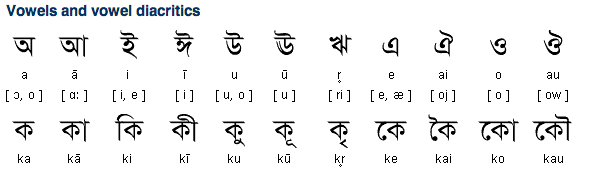
\includegraphics[scale=0.35]{vowels}
  \label{vowels}
\end{figure}
\begin{figure}[h]
  \caption{Consonants in Bengali script.}
  \centering
  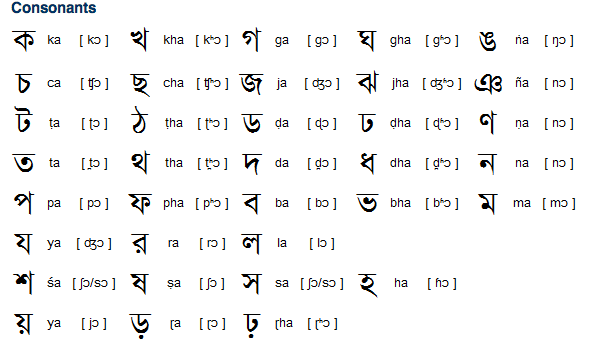
\includegraphics[scale=0.35]{consonants}
  \label{cons}
\end{figure} \\


\newpage


\bibliographystyle{plainnat}
\bibliography{refs}
\label{lastpage}
\end{document}
